\section{海绵构造与 SHA3}\label{sec:8-8}

多年来,基本上所有的抗碰撞哈希函数都是基于 Merkle-Damg{\aa}rd 范式的。然而最近出现了一种新的范式,称为\textbf{海绵构造(sponge construction)}。与 Merkle-Damg{\aa}rd 一样,它也是一个简单的迭代构造,由一个更原始的函数构建而成;但它用的并不是压缩函数 $h:\{0,1\}^{n+\ell}\to\{0,1\}^n$,而是一个置换 $\pi:\{0,1\}^n\to\{0,1\}^n$。我们强调,和分组密码不同,函数 $\pi$ 是没有密钥的。海绵构造和 Merkle-Damg{\aa}rd 构造之间还有两个高层次的区别,我们下面具体说明:
\begin{itemize}
	\item 在消极方面,我们尚不知道如何将海绵构造的抗碰撞性归约到 $\pi$ 的具体安全属性。唯一已知的对海绵构造的分析在理想置换模型下,其中,我们(启发式地)将 $\pi$ 建模为一个真随机的置换 $\Pi$。
	\item 在积极方面,海绵构造被设计成能够灵活和安全地被用于各种抗碰撞性并不是首要需求的应用中。例如,在 \ref{sec:8-7} 节中,我们研究了将哈希函数 $H$ 转换为 PRF $F$ 的几种可行方法。特别地,我们可以看到,当 $H$ 被实例化为一个 Merkle-Damg{\aa}rd 哈希时,简单直观地前缀密钥的想法,即 $F_\mathrm{pre}(k,M):=H(k\,\Vert\,M)$ 并不可行。海绵构造能够避免这些问题:它允许我们将变长的输入哈希成变长的输出,并且,如果我们将 $\pi$ 建模为一个随机置换,那么我们可以声称,对于所有的意图和目的而言,海绵构造都是一个随机函数(我们还将在 \ref{sec:8-10} 节详细讨论)。特别地,当 $H$ 被实例化为一个海绵哈希时,构造 $F_\mathrm{pre}$ 也是安全的。
\end{itemize}

一个被称为 SHA3 的新哈希标准,就是基于海绵构造的。下面,我们先对通用的海绵构造进行介绍和分析,然后讨论 SHA3 的一些技术细节。

\subsection{海绵构造}\label{subsec:8-8-1}

现在,我们更具体地介绍海绵构造。除了指定一个置换 $\pi:\{0,1\}^n\to\{0,1\}^n$ 之外,我们还需要指定两个正整数 $r$ 和 $c$,满足 $n=r+c$。数字 $r$ 被称为海绵构造的\textbf{速率(rate)}:速率越大,计算的速度就越快。数字 $c$ 被称为海绵构造的\textbf{容量(capacity)}:容量越大,安全约束就越强。因此,$r$ 和 $c$ 的不同选择会导致不同的速度/安全性权衡。

海绵构造允许变长的输入。为了哈希一条长消息 $M\in\{0,1\}^{\leq L}$,我们先对 $M$ 后缀一个填充序列,使其长度成为 $r$ 的整数倍,然后将填充后的 $M$ 拆分成一系列 $r$ 比特的分组 $m_1,\dots,m_s$。填充程序的要求是最小化的:它只需要是一个单射。后缀一个形如 $10^*$ 的序列就足以满足需求,尽管如此,SHA3 实际上使用的是形如 $10^*1$ 的填充序列:后者的效果是在最后一个分组中编码速率,并且有助于在使用速率不同的相同海绵构造的应用中分析安全性;然而,我们并不会在这里探讨这些用例。请注意,如果 $M$ 的长度已经是 $r$ 的整数倍,或者接近 $r$ 的整数倍,我们可能就需要添加一个假的分组。

海绵构造也允许变长的输出。因此,除了消息 $M\in\{0,1\}^{\leq L}$ 以外,它还需要输入一个正整数 $v$,后者指定了输出的比特数量。

下面是海绵构造的工作原理:

\vspace{5pt}

\hspace*{5pt} 输入:消息 $M\in\{0,1\}^{\leq L}$ 和期望的输出长度 $v>0$\\
\hspace*{26pt} 输出:一个标签 $h\in\{0,1\}^v$

\vspace{5pt}

\hspace*{5pt} // \emph{吸收阶段}\\
\hspace*{26pt} 对 $M$ 进行填充,并将其拆分为一系列 $r$ 比特分组 $m_1,\dots,m_s\in\{0,1\}^r$\\
\hspace*{26pt} 令 $h\leftarrow 0^n$\\
\hspace*{26pt} 对于 $i=1,\dots,s$:\\
\hspace*{50pt} 令 $m_i'\leftarrow m_i\,\Vert\,0^c\in\{0,1\}^n$\\
\hspace*{50pt} 令 $h\leftarrow\pi(h\oplus m_i')$

\vspace{5pt}

\hspace*{5pt} // \emph{挤出阶段}\\
\hspace*{26pt} 令 $z_1\leftarrow h[0\dots r-1]$\\
\hspace*{26pt} 对于 $i=2,\dots,\lceil v/r\rceil$:\\
\hspace*{50pt} 令 $h\leftarrow\pi(h)$\\
\hspace*{50pt} 令 $z_i\leftarrow h[0\dots r-1]$\\
\hspace*{26pt} 输出 $\left(z_1\,\Vert\,\cdots\,\Vert\,z_{\lceil v/r\rceil}\right)[0\dots v-1]$

\vspace{5pt}
图 \ref{fig:8-11} 可能有助于读者理解该算法。海绵构造的运行可以分为两个阶段:第一阶段被称为``吸收阶段",在这个阶段中,消息分组被``混入"到一个链式变量 $h$ 中;第二阶段被称为``挤出阶段",在该阶段中,输出被从链式变量中``拉出"。请注意,输入分组和输出分组都是 $r$ 比特序列,所以链式变量剩余的 $c$ 个比特不能被攻击者直接篡改甚至看到。这就是海绵构造安全性的来源,也是 $c$ 必须是一个大数的原因。事实上,如果海绵的容量较小,我们就很容易找到它的碰撞(见练习 \ref{exer:8-21})。

\begin{figure}
	\centering
	

\tikzset{every picture/.style={line width=0.75pt}} %set default line width to 0.75pt        

\begin{tikzpicture}[x=0.75pt,y=0.75pt,yscale=-1,xscale=1]
%uncomment if require: \path (0,257); %set diagram left start at 0, and has height of 257

%Shape: Rectangle [id:dp5542688623725909] 
\draw   (40,30) -- (55,30) -- (55,150) -- (40,150) -- cycle ;
%Shape: Rectangle [id:dp7052373194088137] 
\draw   (40,150) -- (55,150) -- (55,190) -- (40,190) -- cycle ;
%Flowchart: Or [id:dp452062836292761] 
\draw   (70,50) .. controls (70,47.24) and (72.24,45) .. (75,45) .. controls (77.76,45) and (80,47.24) .. (80,50) .. controls (80,52.76) and (77.76,55) .. (75,55) .. controls (72.24,55) and (70,52.76) .. (70,50) -- cycle ; \draw   (70,50) -- (80,50) ; \draw   (75,45) -- (75,55) ;
%Rounded Rect [id:dp9974079354662706] 
\draw  [line width=0.4]  (95,33) .. controls (95,31.34) and (96.34,30) .. (98,30) -- (107,30) .. controls (108.66,30) and (110,31.34) .. (110,33) -- (110,187) .. controls (110,188.66) and (108.66,190) .. (107,190) -- (98,190) .. controls (96.34,190) and (95,188.66) .. (95,187) -- cycle ;
%Flowchart: Or [id:dp5914947514518503] 
\draw   (125,50) .. controls (125,47.24) and (127.24,45) .. (130,45) .. controls (132.76,45) and (135,47.24) .. (135,50) .. controls (135,52.76) and (132.76,55) .. (130,55) .. controls (127.24,55) and (125,52.76) .. (125,50) -- cycle ; \draw   (125,50) -- (135,50) ; \draw   (130,45) -- (130,55) ;
%Rounded Rect [id:dp36599491845327137] 
\draw  [line width=0.4]  (150,33) .. controls (150,31.34) and (151.34,30) .. (153,30) -- (162,30) .. controls (163.66,30) and (165,31.34) .. (165,33) -- (165,187) .. controls (165,188.66) and (163.66,190) .. (162,190) -- (153,190) .. controls (151.34,190) and (150,188.66) .. (150,187) -- cycle ;
%Shape: Rectangle [id:dp005089439161285014] 
\draw   (315,30) -- (330,30) -- (330,150) -- (315,150) -- cycle ;
%Shape: Rectangle [id:dp3362181051760911] 
\draw   (315,150) -- (330,150) -- (330,190) -- (315,190) -- cycle ;
%Rounded Rect [id:dp6668484771061065] 
\draw  [line width=0.4]  (370,33) .. controls (370,31.34) and (371.34,30) .. (373,30) -- (382,30) .. controls (383.66,30) and (385,31.34) .. (385,33) -- (385,187) .. controls (385,188.66) and (383.66,190) .. (382,190) -- (373,190) .. controls (371.34,190) and (370,188.66) .. (370,187) -- cycle ;
%Rounded Rect [id:dp58516311055995] 
\draw  [line width=0.4]  (425,33) .. controls (425,31.34) and (426.34,30) .. (428,30) -- (437,30) .. controls (438.66,30) and (440,31.34) .. (440,33) -- (440,187) .. controls (440,188.66) and (438.66,190) .. (437,190) -- (428,190) .. controls (426.34,190) and (425,188.66) .. (425,187) -- cycle ;
%Straight Lines [id:da870690411895882] 
\draw    (55,50) -- (67,50) ;
\draw [shift={(70,50)}, rotate = 180] [fill={rgb, 255:red, 0; green, 0; blue, 0 }  ][line width=0.08]  [draw opacity=0] (5.36,-2.57) -- (0,0) -- (5.36,2.57) -- cycle    ;
%Flowchart: Or [id:dp7426668297118724] 
\draw   (180,50) .. controls (180,47.24) and (182.24,45) .. (185,45) .. controls (187.76,45) and (190,47.24) .. (190,50) .. controls (190,52.76) and (187.76,55) .. (185,55) .. controls (182.24,55) and (180,52.76) .. (180,50) -- cycle ; \draw   (180,50) -- (190,50) ; \draw   (185,45) -- (185,55) ;
%Rounded Rect [id:dp19743989863754363] 
\draw  [line width=0.4]  (205,33) .. controls (205,31.34) and (206.34,30) .. (208,30) -- (217,30) .. controls (218.66,30) and (220,31.34) .. (220,33) -- (220,187) .. controls (220,188.66) and (218.66,190) .. (217,190) -- (208,190) .. controls (206.34,190) and (205,188.66) .. (205,187) -- cycle ;
%Flowchart: Or [id:dp14702351820427184] 
\draw   (235,50) .. controls (235,47.24) and (237.24,45) .. (240,45) .. controls (242.76,45) and (245,47.24) .. (245,50) .. controls (245,52.76) and (242.76,55) .. (240,55) .. controls (237.24,55) and (235,52.76) .. (235,50) -- cycle ; \draw   (235,50) -- (245,50) ; \draw   (240,45) -- (240,55) ;
%Rounded Rect [id:dp9289700961540952] 
\draw  [line width=0.4]  (260,33) .. controls (260,31.34) and (261.34,30) .. (263,30) -- (272,30) .. controls (273.66,30) and (275,31.34) .. (275,33) -- (275,187) .. controls (275,188.66) and (273.66,190) .. (272,190) -- (263,190) .. controls (261.34,190) and (260,188.66) .. (260,187) -- cycle ;
%Straight Lines [id:da596950970496692] 
\draw    (80,50) -- (92,50) ;
\draw [shift={(95,50)}, rotate = 180] [fill={rgb, 255:red, 0; green, 0; blue, 0 }  ][line width=0.08]  [draw opacity=0] (5.36,-2.57) -- (0,0) -- (5.36,2.57) -- cycle    ;
%Straight Lines [id:da8126695347047235] 
\draw    (110,50) -- (122,50) ;
\draw [shift={(125,50)}, rotate = 180] [fill={rgb, 255:red, 0; green, 0; blue, 0 }  ][line width=0.08]  [draw opacity=0] (5.36,-2.57) -- (0,0) -- (5.36,2.57) -- cycle    ;
%Straight Lines [id:da15557526416079437] 
\draw    (135,50) -- (147,50) ;
\draw [shift={(150,50)}, rotate = 180] [fill={rgb, 255:red, 0; green, 0; blue, 0 }  ][line width=0.08]  [draw opacity=0] (5.36,-2.57) -- (0,0) -- (5.36,2.57) -- cycle    ;
%Straight Lines [id:da9893602600371423] 
\draw    (165,50) -- (177,50) ;
\draw [shift={(180,50)}, rotate = 180] [fill={rgb, 255:red, 0; green, 0; blue, 0 }  ][line width=0.08]  [draw opacity=0] (5.36,-2.57) -- (0,0) -- (5.36,2.57) -- cycle    ;
%Straight Lines [id:da14667093283357913] 
\draw    (190,50) -- (202,50) ;
\draw [shift={(205,50)}, rotate = 180] [fill={rgb, 255:red, 0; green, 0; blue, 0 }  ][line width=0.08]  [draw opacity=0] (5.36,-2.57) -- (0,0) -- (5.36,2.57) -- cycle    ;
%Straight Lines [id:da6813337200107608] 
\draw    (220,50) -- (232,50) ;
\draw [shift={(235,50)}, rotate = 180] [fill={rgb, 255:red, 0; green, 0; blue, 0 }  ][line width=0.08]  [draw opacity=0] (5.36,-2.57) -- (0,0) -- (5.36,2.57) -- cycle    ;
%Straight Lines [id:da8347713066945073] 
\draw    (245,50) -- (257,50) ;
\draw [shift={(260,50)}, rotate = 180] [fill={rgb, 255:red, 0; green, 0; blue, 0 }  ][line width=0.08]  [draw opacity=0] (5.36,-2.57) -- (0,0) -- (5.36,2.57) -- cycle    ;
%Straight Lines [id:da3017178302912422] 
\draw    (75,25) -- (75,42) ;
\draw [shift={(75,45)}, rotate = 270] [fill={rgb, 255:red, 0; green, 0; blue, 0 }  ][line width=0.08]  [draw opacity=0] (5.36,-2.57) -- (0,0) -- (5.36,2.57) -- cycle    ;
%Straight Lines [id:da8587452708873555] 
\draw    (130,25) -- (130,42) ;
\draw [shift={(130,45)}, rotate = 270] [fill={rgb, 255:red, 0; green, 0; blue, 0 }  ][line width=0.08]  [draw opacity=0] (5.36,-2.57) -- (0,0) -- (5.36,2.57) -- cycle    ;
%Straight Lines [id:da4230499595507906] 
\draw    (185,25) -- (185,42) ;
\draw [shift={(185,45)}, rotate = 270] [fill={rgb, 255:red, 0; green, 0; blue, 0 }  ][line width=0.08]  [draw opacity=0] (5.36,-2.57) -- (0,0) -- (5.36,2.57) -- cycle    ;
%Straight Lines [id:da8314749511251045] 
\draw    (240,25) -- (240,42) ;
\draw [shift={(240,45)}, rotate = 270] [fill={rgb, 255:red, 0; green, 0; blue, 0 }  ][line width=0.08]  [draw opacity=0] (5.36,-2.57) -- (0,0) -- (5.36,2.57) -- cycle    ;
%Straight Lines [id:da4458343142601504] 
\draw    (55,170) -- (92,170) ;
\draw [shift={(95,170)}, rotate = 180] [fill={rgb, 255:red, 0; green, 0; blue, 0 }  ][line width=0.08]  [draw opacity=0] (5.36,-2.57) -- (0,0) -- (5.36,2.57) -- cycle    ;
%Straight Lines [id:da05886256165116843] 
\draw    (110,170) -- (147,170) ;
\draw [shift={(150,170)}, rotate = 180] [fill={rgb, 255:red, 0; green, 0; blue, 0 }  ][line width=0.08]  [draw opacity=0] (5.36,-2.57) -- (0,0) -- (5.36,2.57) -- cycle    ;
%Straight Lines [id:da22933289791805644] 
\draw    (165,170) -- (202,170) ;
\draw [shift={(205,170)}, rotate = 180] [fill={rgb, 255:red, 0; green, 0; blue, 0 }  ][line width=0.08]  [draw opacity=0] (5.36,-2.57) -- (0,0) -- (5.36,2.57) -- cycle    ;
%Straight Lines [id:da7356216235252535] 
\draw    (220,170) -- (257,170) ;
\draw [shift={(260,170)}, rotate = 180] [fill={rgb, 255:red, 0; green, 0; blue, 0 }  ][line width=0.08]  [draw opacity=0] (5.36,-2.57) -- (0,0) -- (5.36,2.57) -- cycle    ;
%Straight Lines [id:da7856904185972291] 
\draw    (275,170) -- (312,170) ;
\draw [shift={(315,170)}, rotate = 180] [fill={rgb, 255:red, 0; green, 0; blue, 0 }  ][line width=0.08]  [draw opacity=0] (5.36,-2.57) -- (0,0) -- (5.36,2.57) -- cycle    ;
%Straight Lines [id:da525685135110235] 
\draw    (330,170) -- (367,170) ;
\draw [shift={(370,170)}, rotate = 180] [fill={rgb, 255:red, 0; green, 0; blue, 0 }  ][line width=0.08]  [draw opacity=0] (5.36,-2.57) -- (0,0) -- (5.36,2.57) -- cycle    ;
%Straight Lines [id:da0547341588479997] 
\draw    (385,170) -- (422,170) ;
\draw [shift={(425,170)}, rotate = 180] [fill={rgb, 255:red, 0; green, 0; blue, 0 }  ][line width=0.08]  [draw opacity=0] (5.36,-2.57) -- (0,0) -- (5.36,2.57) -- cycle    ;
%Straight Lines [id:da24635646326301108] 
\draw    (275,50) -- (312,50) ;
\draw [shift={(315,50)}, rotate = 180] [fill={rgb, 255:red, 0; green, 0; blue, 0 }  ][line width=0.08]  [draw opacity=0] (5.36,-2.57) -- (0,0) -- (5.36,2.57) -- cycle    ;
%Straight Lines [id:da5909600445720702] 
\draw    (330,50) -- (367,50) ;
\draw [shift={(370,50)}, rotate = 180] [fill={rgb, 255:red, 0; green, 0; blue, 0 }  ][line width=0.08]  [draw opacity=0] (5.36,-2.57) -- (0,0) -- (5.36,2.57) -- cycle    ;
%Straight Lines [id:da25290311891602046] 
\draw    (385,50) -- (422,50) ;
\draw [shift={(425,50)}, rotate = 180] [fill={rgb, 255:red, 0; green, 0; blue, 0 }  ][line width=0.08]  [draw opacity=0] (5.36,-2.57) -- (0,0) -- (5.36,2.57) -- cycle    ;
%Straight Lines [id:da24008038895508155] 
\draw    (440,50) -- (460,50) -- (460,28) ;
\draw [shift={(460,25)}, rotate = 90] [fill={rgb, 255:red, 0; green, 0; blue, 0 }  ][line width=0.08]  [draw opacity=0] (5.36,-2.57) -- (0,0) -- (5.36,2.57) -- cycle    ;
%Straight Lines [id:da1596470859914647] 
\draw    (350,50) -- (350,28) ;
\draw [shift={(350,25)}, rotate = 90] [fill={rgb, 255:red, 0; green, 0; blue, 0 }  ][line width=0.08]  [draw opacity=0] (5.36,-2.57) -- (0,0) -- (5.36,2.57) -- cycle    ;
%Straight Lines [id:da26264968581498205] 
\draw    (405,50) -- (405,28) ;
\draw [shift={(405,25)}, rotate = 90] [fill={rgb, 255:red, 0; green, 0; blue, 0 }  ][line width=0.08]  [draw opacity=0] (5.36,-2.57) -- (0,0) -- (5.36,2.57) -- cycle    ;
%Straight Lines [id:da012331121329425043] 
\draw  [dash pattern={on 4.5pt off 4.5pt}]  (295,10) -- (295,215) ;
%Straight Lines [id:da8548139600256164] 
\draw    (30,30) -- (30,150) ;
\draw [shift={(30,150)}, rotate = 270] [color={rgb, 255:red, 0; green, 0; blue, 0 }  ][line width=0.75]    (0,3.35) -- (0,-3.35)(6.56,-1.97) .. controls (4.17,-0.84) and (1.99,-0.18) .. (0,0) .. controls (1.99,0.18) and (4.17,0.84) .. (6.56,1.97)   ;
\draw [shift={(30,30)}, rotate = 90] [color={rgb, 255:red, 0; green, 0; blue, 0 }  ][line width=0.75]    (0,3.35) -- (0,-3.35)(6.56,-1.97) .. controls (4.17,-0.84) and (1.99,-0.18) .. (0,0) .. controls (1.99,0.18) and (4.17,0.84) .. (6.56,1.97)   ;
%Straight Lines [id:da3516341856026399] 
\draw    (30,150) -- (30,190) ;
\draw [shift={(30,190)}, rotate = 270] [color={rgb, 255:red, 0; green, 0; blue, 0 }  ][line width=0.75]    (0,3.35) -- (0,-3.35)(6.56,-1.97) .. controls (4.17,-0.84) and (1.99,-0.18) .. (0,0) .. controls (1.99,0.18) and (4.17,0.84) .. (6.56,1.97)   ;
\draw [shift={(30,150)}, rotate = 90] [color={rgb, 255:red, 0; green, 0; blue, 0 }  ][line width=0.75]    (0,3.35) -- (0,-3.35)(6.56,-1.97) .. controls (4.17,-0.84) and (1.99,-0.18) .. (0,0) .. controls (1.99,0.18) and (4.17,0.84) .. (6.56,1.97)   ;
%Shape: Circle [id:dp9825549442373853] 
\draw  [fill={rgb, 255:red, 0; green, 0; blue, 0 }  ,fill opacity=1 ] (348.5,50) .. controls (348.5,49.17) and (349.17,48.5) .. (350,48.5) .. controls (350.83,48.5) and (351.5,49.17) .. (351.5,50) .. controls (351.5,50.83) and (350.83,51.5) .. (350,51.5) .. controls (349.17,51.5) and (348.5,50.83) .. (348.5,50) -- cycle ;
%Shape: Circle [id:dp3708606046839278] 
\draw  [fill={rgb, 255:red, 0; green, 0; blue, 0 }  ,fill opacity=1 ] (403.5,50) .. controls (403.5,49.17) and (404.17,48.5) .. (405,48.5) .. controls (405.83,48.5) and (406.5,49.17) .. (406.5,50) .. controls (406.5,50.83) and (405.83,51.5) .. (405,51.5) .. controls (404.17,51.5) and (403.5,50.83) .. (403.5,50) -- cycle ;

% Text Node
\draw (47.5,90) node    {$0$};
% Text Node
\draw (47.5,170) node    {$0$};
% Text Node
\draw (102.5,110) node    {$f$};
% Text Node
\draw (157.5,110) node    {$f$};
% Text Node
\draw (212.5,110) node    {$f$};
% Text Node
\draw (267.5,110) node    {$f$};
% Text Node
\draw (377.5,110) node    {$f$};
% Text Node
\draw (432.5,110) node    {$f$};
% Text Node
\draw (75,21.6) node [anchor=south] [inner sep=0.75pt]    {$m_{1}$};
% Text Node
\draw (130,21.6) node [anchor=south] [inner sep=0.75pt]    {$m_{2}$};
% Text Node
\draw (185,21.6) node [anchor=south] [inner sep=0.75pt]    {$m_{3}$};
% Text Node
\draw (240,21.6) node [anchor=south] [inner sep=0.75pt]    {$m_{4}$};
% Text Node
\draw (350,21.6) node [anchor=south] [inner sep=0.75pt]    {$z_{1}$};
% Text Node
\draw (405,21.6) node [anchor=south] [inner sep=0.75pt]    {$z_{2}$};
% Text Node
\draw (460,21.6) node [anchor=south] [inner sep=0.75pt]    {$z_{3}$};
% Text Node
\draw (28,90) node [anchor=east] [inner sep=1pt]  [font=\small] [align=left] {$r$ bits};
% Text Node
\draw (28,170) node [anchor=east] [inner sep=1pt]  [font=\small] [align=left] {$c$ bits};
% Text Node
\draw (150,217) node [anchor=south] [inner sep=0.75pt]   [align=left] {\textbf{吸收阶段}};
% Text Node
\draw (380,217) node [anchor=south] [inner sep=0.75pt]   [align=left] {\textbf{挤出阶段}};


\end{tikzpicture}
	\caption{海绵构造}
	\label{fig:8-11}
\end{figure}

在 SHA3 标准中,海绵构造被用作抗碰撞哈希,其输出长度被固定为一个 $v\leq r$ 的值,因此,在挤出阶段,它只是输出吸收阶段的输出值 $h$ 的前 $v$ 比特。现在,我们将证明,如果假设 $2^c$ 和 $2^v$ 都是超多项式的,那么该版本的海绵构造在理想置换模型下就是抗碰撞的。

\begin{theorem}\label{theo:8-6}
假设 $H$ 是由置换 $\pi:\{0,1\}^n\to\{0,1\}^n$ 得到的哈希函数,其容量为 $c$,速率为 $r$(所以有 $n=r+c$),输出长度为$v\leq r$。在理想置换模型下,$\pi$ 被建模为一个随机置换 $\Pi$,那么如果假设 $2^v$ 和 $2^c$ 都是超多项式的,则哈希函数 $H$ 是抗碰撞的。
\begin{quote}
特别地,对于每个碰撞查找对手 $\mathcal{A}$,如果理想置换查询的数量与 $\mathcal{A}$ 的输出消息中的 $r$ 比特分组的数量之和被 $q$ 约束,那么:
\end{quote}
\[
\mathrm{CR}^\mathrm{ic}\mathsf{adv}[\mathcal{A},H]
\leq
\frac{q(q-1)}{2^v}+\frac{q(q+1)}{2^c}
\]
\end{theorem}

\begin{proof}
与定理 \ref{theo:8-4} 的证明一样,我们假设我们的碰撞查找对手是``合理的",即它所发起的理想置换查询都与其输出相关。通过迫使对手在其输出消息上计算哈希函数(如果它尚未这样做的话),我们就可以轻松地将任意对手转化为一个合理的对手。正如我们的定义,$q$ 将是我们的合理对手所发起的理想置换查询总数的一个上界。所以从现在开始,我们假设合理的对手 $\mathcal{A}$ 最多可以发起 $q$ 次查询,并且我们约束这样的 $\mathcal{A}$ 在其查询过程中发现任何可以``组装"成碰撞的东西的概率(我们在下面会更精确地说明)。

我们还假设,\emph{没有任何查询是冗余的}。这意味着,如果对手已经对 $\mathpzc{a}$ 进行了一次 $\Pi$-查询并得到 $\mathpzc{b}=\Pi(\mathpzc{a})$,那么对手就不会再对 $\mathpzc{b}$ 进行 $\Pi^{-1}$-查询,也不会再对 $\mathpzc{a}$ 进行 $\Pi$-查询;类似地,如果对手对 $\mathpzc{b}$ 进行了一次 $\Pi^{-1}$-查询并得到 $\mathpzc{a}=\Pi^{-1}(\mathpzc{b})$,它就永远不会再对 $\mathpzc{a}$ 进行 $\Pi$-查询,也不会再对 $\mathpzc{b}$ 进行 $\Pi^{-1}$-查询。当然,对手没有必要进行这种冗余的查询,这也是我们排除它们的原因;此外,这样做将会极大简化我们证明过程中的记录。

具体地说,这有助于把对手的攻击过程想象成一个有向图 $G$ 的构建过程。$G$ 中的节点由所有长度为 $n$ 比特的 $2^n$ 个序列的集合组成。图 $G$ 在开始时并没有边,$\mathcal{A}$ 的每一次查询都会给图增加一条边:如果 $\mathcal{A}$ 对 $\mathpzc{a}$ 进行了一次 $\Pi$-查询并产生了 $\mathpzc{b}$,或者对 $\mathpzc{b}$ 进行了一次 $\Pi^{-1}$-查询并产生了 $\mathpzc{a}$,就会增加一条边 $\mathpzc{a}\to\mathpzc{b}$。请注意,如果我们有一条边 $\mathpzc{a}\to\mathpzc{b}$,就一定有 $\Pi(\mathpzc{a})=\mathpzc{b}$,不管这条边是来自一个 $\Pi$-查询,还是来自一个 $\Pi^{-1}$-查询。我们称通过 $\Pi$-查询添加的边是\textbf{前向边(forward edge)},通过 $\Pi^{-1}$-查询添加的边是\textbf{后向边(back edge)}。

请注意,我们假设对手不做冗余的查询,这也就意味着一条边只会被添加到图中一次,而它的类型是由添加该边的查询类型唯一决定的。

接下来,我们在图中定义一种特殊类型的路径,它对应于对海绵构造的计算。对于一个 $n$ 比特的序列 $\mathpzc{z}$,令 $R(\mathpzc{z})$ 是 $\mathpzc{z}$ 的前 $r$ 比特,$C(\mathpzc{z})$ 是 $\mathpzc{z}$ 的后 $c$ 比特。我们称 $R(\mathpzc{z})$ 为 \textbf{$\mathpzc{z}$ 的 $R$-部分 ($R$-part of $\mathpzc{z}$)},$C(\mathpzc{z})$ 为 \textbf{$\mathpzc{z}$ 的 $C$-部分 ($C$-part of $\mathpzc{z}$)}。对于 $s>1$,一个\textbf{长度为 $s$ 的 $C$-路径 ($C$-path of length $s$)}指的是一个由 $2s$ 个结点组成的序列:
\[
\mathpzc{a}_0,\mathpzc{b}_1,\mathpzc{a}_1,\mathpzc{b}_2,\mathpzc{a}_2,\dots,\mathpzc{b}_{s-1},\mathpzc{a}_{s-1},\mathpzc{b}_s
\]
其中:
\begin{itemize}
	\item $C(\mathpzc{a}_0)=0^c$,此外,对于 $i=1,\dots,s-1$,我们有 $C(\mathpzc{b}_i)=C(\mathpzc{a}_i)$;并且,
	\item 对于 $i=1,\dots,s$,$G$ 包含边 $\mathpzc{a}_{i-1}\to\mathpzc{b}_i$。
\end{itemize}
对于这样的一条路径 $p$,$p$ 的\textbf{消息}被定义为 $(m_0,\dots,m_{s-1})$,其中:
\[
m_0:=R(\mathpzc{a}_0),
\qquad
m_i:=R(\mathpzc{b}_i)\oplus R(\mathpzc{a}_i)
\quad\text{for}\quad
i=1,\dots,s-1
\]
而 $p$ 的\textbf{结果}被定义为 $m_s:=R(\mathpzc{b}_s)$。这样一条 $C$-路径 $p$ 对应于在消息 $(m_0,\dots,m_{s-1})$ 上对海绵构造进行计算,并获得(未截短的)输出 $m_s$。 我们可以把这样的路径写成:
\begin{equation}\label{eq:8-12}
m_0|\mathpzc{a}_0\longrightarrow
\mathpzc{b}_1|m_1|\mathpzc{a}_1\longrightarrow\cdots\longrightarrow
\mathpzc{b}_{s-2}|m_{s-2}|\mathpzc{a}_{s-2}\longrightarrow
\mathpzc{b}_{s-1}|m_{s-1}|\mathpzc{a}_{s-1}\longrightarrow
\mathpzc{b}_{s}|m_{s}
\end{equation}
下图展示了一条长度为 $3$ 的$C$-路径。

\begin{figure*}[h!]
  \centering
  \tikzset{every picture/.style={line width=0.75pt}} %set default line width to 0.75pt        

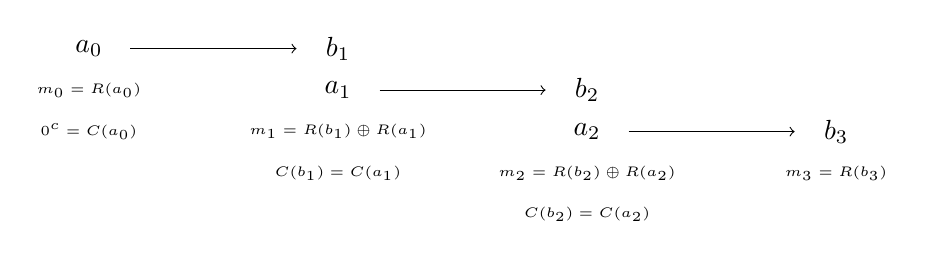
\begin{tikzpicture}[x=0.75pt,y=0.75pt,yscale=-1,xscale=1]
%uncomment if require: \path (0,300); %set diagram left start at 0, and has height of 300

%Straight Lines [id:da8110716189627085] 
\draw  [->]  (70,20) -- (150,20) ;
%Straight Lines [id:da7276012637365663] 
\draw  [->]  (190,40) -- (270,40) ;
%Straight Lines [id:da8434556424917563] 
\draw  [->]  (310,60) -- (390,60) ;

% Text Node
\draw (50.02,20) node    {$\mathpzc{a}_{0}$};
% Text Node
\draw (170,20) node    {$\mathpzc{b}_{1}$};
% Text Node
\draw (170,40) node    {$\mathpzc{a}_{1}$};
% Text Node
\draw (290,40) node    {$\mathpzc{b}_{2}$};
% Text Node
\draw (290,60) node    {$\mathpzc{a}_{2}$};
% Text Node
\draw (410,60) node    {$\mathpzc{b}_{3}$};
% Text Node
\draw (50,40) node  [font=\tiny]  {$m_{0}=R(\mathpzc{a}_{0})$};
% Text Node
\draw (50,60) node  [font=\tiny]  {$0^{c}=C(\mathpzc{a}_{0})$};
% Text Node
\draw (170,60) node  [font=\tiny]  {$m_{1}=R(\mathpzc{b}_{1}) \oplus R(\mathpzc{a}_{1})$};
% Text Node
\draw (170,80) node  [font=\tiny]  {$C(\mathpzc{b}_{1})=C(\mathpzc{a}_{1})$};
% Text Node
\draw (290,80) node  [font=\tiny]  {$m_{2}=R(\mathpzc{b}_{2}) \oplus R(\mathpzc{a}_{2})$};
% Text Node
\draw (290,100) node  [font=\tiny]  {$C(\mathpzc{b}_{2})=C(\mathpzc{a}_{2})$};
% Text Node
\draw (410,80) node  [font=\tiny]  {$m_{3}=R(\mathpzc{b}_{3})$};


\end{tikzpicture}
\end{figure*}

\noindent
该路径有消息 $(m_0,m_1,m_2)$ 和结果 $m_3$。使用式 \ref{eq:8-12} 中的符号,我们可以把该路径写成:
\[
m_0|\mathpzc{a}_0\longrightarrow
\mathpzc{b}_1|m_1|\mathpzc{a}_1\longrightarrow
\mathpzc{b}_2|m_2|\mathpzc{a}_2\longrightarrow
\mathpzc{b}_3|m_3
\]

现在我们可以从图 $G$ 的角度来说明碰撞是什么样子的。在有向图中,碰撞就是一对在不同消息上的 $C$-路径,但它们结果的前 $v$ 比特是一致的(回忆一下,我们有 $v\leq r$)。我们称这样的一对路径是\emph{相撞的 (colliding)}。

为了分析找到一对相撞的路径的概率,我们还需要定义另一个概念。令 $p$ 和 $p'$ 是不同消息上的两条 $C$-路径,它们的最后一条边分别是 $\mathpzc{a}_{s-1}\to\mathpzc{b}_s$ 和 $\mathpzc{a}_{t-1}'\to\mathpzc{b}_t'$。如果:
\begin{enumerate}[(i)]
	\item $\mathpzc{a}_{s-1} = \mathpzc{a}_{t-1}'$,或者
	\item $p$ 或 $p'$ 中存在某条边是后向边
\end{enumerate}
我们就称路径对 $p$ 和 $p'$ 是\emph{有问题的 (problematic)}。

令 $W$ 是 $\mathcal{A}$ 发现一对相撞的路径的事件,并令 $Z$ 是 $\mathcal{A}$ 发现一对有问题的路径的事件。那么我们有:
\begin{equation}\label{eq:8-13}
\Pr[W]\leq\Pr[Z]+\Pr[W\land\lnot Z]
\end{equation}

首先,我们计算 $\Pr[W\land\lnot Z]$ 的约束。对于一个 $n$ 比特的序列 $\mathpzc{z}$,令 $V(\mathpzc{z})$ 是 $\mathpzc{z}$ 的前 $v$ 比特,我们可以称 $V(\mathpzc{z})$ 为 \textbf{$\mathpzc{z}$ 的 $V$-部分 ($V$-part of $\mathpzc{z}$)}。假设 $\mathcal{A}$ 能够找到一对没有问题的相撞路径。根据定义,这两条路径的最终边对应于不同输入上的$\Pi$-查询,产生的输出的 $V$-部分也是一致的。也就是说,如果事件 $W\land\lnot Z$ 发生,那么情况一定是,在某一时刻,$\mathcal{A}$ 对互不相同的输入 $\mathpzc{a}$ 和 $\mathpzc{a}'$ 发起了两次 $\Pi$-查询并产生输出 $b$ 和 $b'$,满足 $V(\mathpzc{b})=V(\mathpzc{b}')$。我们可以使用联合约束:对于每对索引 $i<j$,记 $X_{ij}$ 为事件:第 $i$ 次查询是对某个值(比如 $\mathpzc{a}$)的 $\Pi$-查询,产生 $\mathpzc{b}=\Pi(\mathpzc{a})$,第 $j$ 次查询是对另一个值 $\mathpzc{a}'\neq\mathpzc{a}$ 的 $\Pi$-查询,产生 $\mathpzc{b}'=\Pi(\mathpzc{a}')$,且满足 $V(\mathpzc{b})=V(\mathpzc{b}')$。如果我们固定 $i$ 和 $j$,固定 $\mathcal{A}$ 的硬币,并且固定第 $j$ 次查询之前的所有查询的输出,那么 $\mathpzc{a}$、$\mathpzc{b}$ 和 $\mathpzc{a}'$ 的值必然都是固定的,但 $\mathpzc{b}'$ 的值将均匀分布在一个大小至少为 $2^n-j+1$ 的集合上。为了使 $V(\mathpzc{b})=V(\mathpzc{b}')$ 成立,$\mathpzc{b}'$ 必须满足其前 $v$ 比特与 $\mathpzc{b}$ 相同,而这有 $2^{n-v}$ 种可能性,因此我们有:
\[
\Pr[X_{ij}]\leq\frac{2^{n-v}}{2^n-j+1}
\]
参考定理 \ref{theo:8-4} 的证明中的式 \ref{eq:8-5},通过一个与之类似的计算,我们就能推出:
\begin{equation}\label{eq:8-14}
\Pr[W\land\lnot Z]\leq
\frac{q(q-1)}{2^v}
\end{equation}
  
其次,我们计算 $\Pr[Z]$ 的约束,即 $\mathcal{A}$ 找到一对有问题的路径的概率。分析的技术核心如下:

\vspace{5pt}

\textbf{主要声称:}\emph{如果事件 $Z$ 发生,那么下面两种情况之一发生:
\begin{quote}
\begin{enumerate}[(E1)]
	\item 某个查询产生了一个 $C$-部分为 $0^c$ 的输出,或
	\item 两个不同的查询所产生输出的 $C$-部分相等。
\end{enumerate}
\end{quote}
}
更具体地说,(E1) 情况意味着 $\mathcal{A}$ 发起了一个如下形式的查询:
\begin{quote}
\begin{enumerate}[(i)]
	\item 对某个值 $\mathpzc{b}$ 的 $\Pi^{-1}$-查询,满足 $C(\Pi^{-1}(\mathpzc{b}))=0^c$,或者
	\item 对某个值 $\mathpzc{a}$ 的 $\Pi$-查询,满足 $C(\Pi(\mathpzc{a}))=0^c$。
\end{enumerate}
\end{quote}
而 (E2) 情况意味着 $\mathcal{A}$ 发起了一对如下形式的查询:
\begin{quote}
\begin{enumerate}[(i)]
	\item 对某个值 $\mathpzc{a}$ 的 $\Pi$-查询和对某个值 $\mathpzc{b}$ 的 $\Pi^{-1}$-查询,满足 $C(\Pi(\mathpzc{a}))=C(\Pi^{-1}(\mathpzc{b}))$,或者
	\item 对两个不同值 $\mathpzc{a}$ 和 $\mathpzc{a}'$ 的 $\Pi$-查询,满足 $C(\Pi(\mathpzc{a}))=C(\Pi(\mathpzc{a}'))$。
\end{enumerate}
\end{quote}

首先,假设 $\mathcal{A}$ 能够找到一对有问题的路径,而且其中一条路径包含一条后向边。那么,在执行的最后,存在一条包含一条或多条后向边的 $C$-路径。令 $p$ 表示这样一条长度最短的路径,如式 \ref{eq:8-12} 所示的那样。我们可以观察到,$p$ 中的最后一条边是一条后边,而 $p$ 中的所有其他边(如果有的话)都是前向边。事实上,如果情况不是这样,那么我们可以从 $p$ 中删除这条边,得到一条包含后向边的更短的 $C$-路径,但这与 $p$ 是这种类型的最短路径的假设相矛盾。从这个观察中,我们可以看到下面两种情况中的一种发生:
\begin{itemize}
	\item $s=1$,并且情况 (E1) 在对 $\mathpzc{b}_1$ 的 $\Pi^{-1}$-查询上发生,或者
	\item $s>1$,并且情况 (E2) 在对 $\mathpzc{b}_s$ 的 $\Pi^{-1}$-查询和对 $\mathpzc{a}_{s-2}$ 的 $\Pi$-查询上发生。
\end{itemize}

其次,假设 $\mathcal{A}$ 能够找到一对有问题的路径,且它们都不包含任何后向边。我们记这对路径为 $p$ 和 $p'$。这种情况下的论证有点类似于 Merkle-Damg{\aa}rd 分析中的``逆向行走"。将 $p$ 写成式 \ref{eq:8-12} 的形式,并将 $p'$ 写成:
\[
m_0'|\mathpzc{a}_0'\longrightarrow
\mathpzc{b}_1'|m_1'|\mathpzc{a}_1'\longrightarrow\cdots\longrightarrow
\mathpzc{b}_{t-2}'|m_{t-2}'|\mathpzc{a}_{t-2}'\longrightarrow
\mathpzc{b}_{t-1}'|m_{t-1}'|\mathpzc{a}_{t-1}'\longrightarrow
\mathpzc{b}_{t}'|m_{t}'
\]
我们已有假设 $(m_0,\dots,m_{s-1})\neq(m_0',\dots,m_{t-1}')$,但是 $\mathpzc{a}_{s-1}=\mathpzc{a}_{t-1}'$,并且这些边都不是后向边。我们还假设我们所选择的路径都是最短的,在这个意义上,$s+t$ 在所有这种类型的 $C$-路径中是最小的。另外,我们假设 $s\leq t$(如有必要,可以互换它们)。于是有以下几种情况:
\begin{enumerate}
	\item $s=1$ 且 $t=1$。这种情况是不可能的,因为在这种情况下,路径就是 $m_0|\mathpzc{a}_0\to\mathpzc{b}_1|m_1$ 和 $m_0'|\mathpzc{a}_0'\to\mathpzc{b}_1'|m_1'$,但 $m_0\neq m_0'$ 和 $\mathpzc{a}_0=\mathpzc{a}_0'$ 不可能同时成立。
	\item $s=1$ 且 $t\geq 2$。在这种情况下,我们有 $\mathpzc{a}_0=\mathpzc{b}_{t-1}'$,所以 情况 (E1) 在对 $\mathpzc{a}_{t-2}'$ 的 $\Pi$-查询上发生。
	\item $s\geq 2$ 且 $t\geq 2$。考虑倒数第二条边,即前向边:
	\[
	\mathpzc{a}_{s-2}\to\mathpzc{b}_{s-1}|m_{s-1}|\mathpzc{a}_{s-1}
	\]
	和
	\[
	\mathpzc{a}_{t-2}'\to\mathpzc{b}_{t-1}'|m_{t-1}'|\mathpzc{a}_{t-1}'
	\]
	我们已经假设 $\mathpzc{a}_{s-1}=\mathpzc{a}_{t-1}'$。因此,$\mathpzc{b}_{s-1}$ 和 $\mathpzc{b}_{t-1}'$ 的 $C$-部分是相等的,并且它们 $R$-部分的差为 $m_{s-1}\oplus m_{t-1}'$。有以下两种子情况:
	\begin{enumerate}[(a)]
		\item $m_{s-1}=m_{t-1}'$。我们声称,这种情况是不可能的。事实上,在这种情况下,我们有 $\mathpzc{b}_{s-1}= \mathpzc{b}_{t-1}'$,继而有 $\mathpzc{a}_{s-2}=\mathpzc{a}_{t-2}'$,然而,截短的消息 $(m_0,\dots,m_{s-2})$ 和 $(m_0',\dots,m_{t-2}')$ 是不同的。因此,我们可以简单地扔掉两条路径中的最后一条边,得到一对较短的路径,而这与 $s+t$ 的最小性矛盾。
		\item $m_{s-1}\neq m_{t-1}'$。在这种情况下,我们知道:$\mathpzc{b}_{s-1}$ 和 $\mathpzc{b}_{t-1}'$ 的 $C$-部分是相同的,但它们的 $R$-部分不同,因此 $\mathpzc{a}_{s-2}\neq\mathpzc{a}_{t-2}'$。因此,情况 (E2) 在对 $\mathpzc{a}_{s-2}$ 和 $\mathpzc{a}_{t-2}'$ 的 $\Pi$-查询上发生。
	\end{enumerate}
\end{enumerate}

这证明了我们上面的主要声称。现在,我们可以转而讨论情况 (E1) 或 (E2) 发生概率的约束。其实我们已经至少做过两次类似的计算了,一次是在上面,我们以此得到了式 \ref{eq:8-14};另一次是在之前的定理 \ref{theo:8-4} 的证明中。与式 \ref{eq:8-14} 唯一不同的是,我们现在是在计算 $C$-部分上的碰撞,而且我们有一种新的``碰撞"类型要计算,即 (E1) 中的``撞到 $0^c$"。我们把它留给读者来验证:
\begin{equation}\label{eq:8-15}
\Pr[Z]\leq\frac{q(q+1)}{2^c}
\end{equation}
于是,根据式 \ref{eq:8-13},\ref{eq:8-14} 和 \ref{eq:8-15},该定理得证。
\end{proof}

\subsection{案例研究:SHA3,SHAKE256 和 SHAKE512}\label{subsec:8-8-2}

NIST 的 SHA3 标准规定了一个基于海绵构造的哈希函数系列。这些哈希函数的核心是一个叫做 Keccak 的置换,它能将 $1600$ 比特的序列映射为 $1600$ 比特的序列。我们用 Keccak[$c$] 表示从 Keccak 派生出的容量为 $c$ 的,使用 $10^*1$ 填充规则的海绵构造。它其实是一个接受两个输入——消息 $m$ 和输出长度 $v$——的函数。这里,$\mathrm{Keccak}[c](m,v)$ 的输入 $m$ 是一个任意的比特序列,而它的输出是一个 $v$ 比特的序列。

我们不会描述 Keccak 置换的内部工作原理,感兴趣的读者可以从 SHA3 标准中找到它。我们只在这里介绍标准化的若干参数选择。该标准规定了四个定长输出和两个变长输出的哈希函数。

以下是四个定长输出的哈希函数:
\begin{itemize}
	\item $\mathrm{SHA3}\text{-}224(m)=\mathrm{Keccak}[448](m\,\Vert\,01,224)$
	\item $\mathrm{SHA3}\text{-}256(m)=\mathrm{Keccak}[512](m\,\Vert\,01,256)$
	\item $\mathrm{SHA3}\text{-}384(m)=\mathrm{Keccak}[768](m\,\Vert\,01,384)$
	\item $\mathrm{SHA3}\text{-}512(m)=\mathrm{Keccak}[1024](m\,\Vert\,01,512)$
\end{itemize}
注意附加在消息后的两个额外的填充比特。注意,在每种情况下,容量 $c$ 都等于输出长度 $v$ 的两倍。因此,随着输出长度的增长,容量所提供的安全性也在增长,而速率(即散列速度)在下降。

以下是两个变长输出的哈希函数:
\begin{itemize}
	\item $\mathrm{SHAKE128}(m,v)=\mathrm{Keccak}[256](m\,\Vert\,1111,v)$
	\item $\mathrm{SHAKE256}(m,v)=\mathrm{Keccak}[512](m\,\Vert\,1111,v)$
\end{itemize}

注意附加在消息后的四个额外的填充比特。两者之间唯一的区别是容量大小,它会影响到速度和安全性。各种填充比特和 $10^*1$ 的填充规则确保这六个函数的行为是相互独立的。
